\section{Accelerating Text Classifier}

\subsection{Acheived Performance}

\begin{figure}[h]
    \centering
    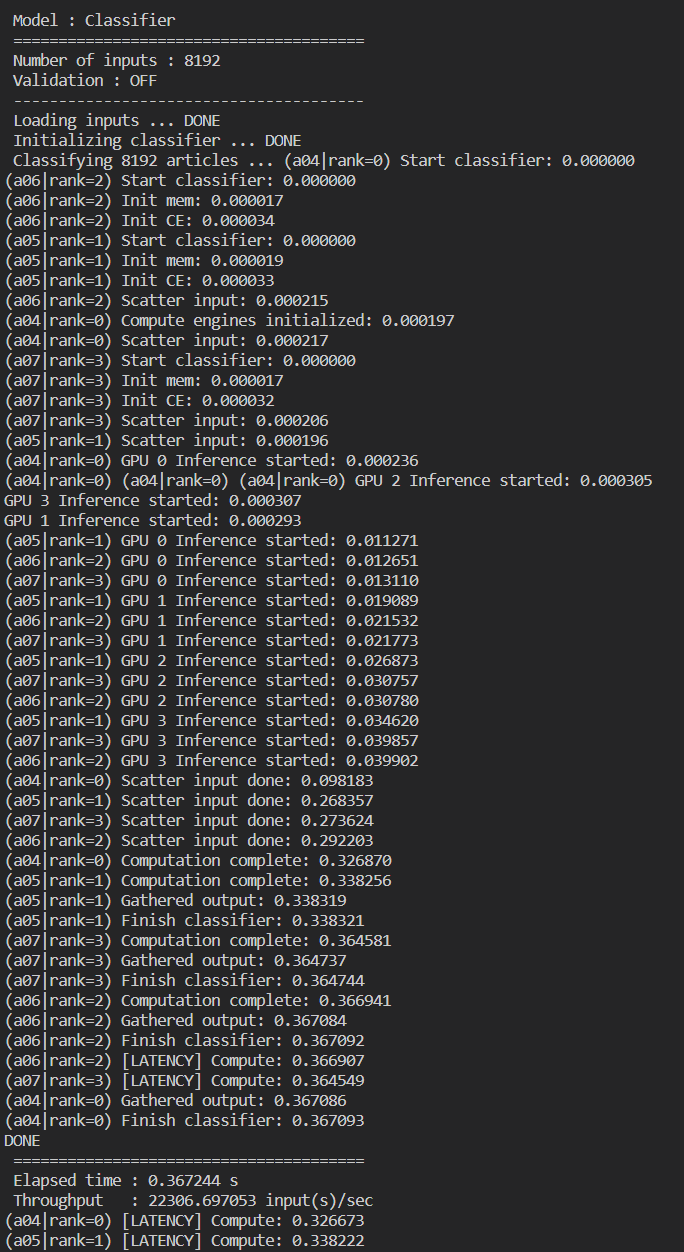
\includegraphics[width=0.6\textwidth]{imgs/best_record.png}
    \caption{The best record of my implementation.}
    \label{fig:best_record}
\end{figure}

총 8192개의 input을 4개 노드에서 연산하도록 하여 최고 
\textbf{22306.697053 input(s)/sec}의 성능을 달성하였다[Fig.~\ref{fig:best_record}].

\subsection{Implementation}
Root 노드는 MPI를 이용하여 나머지 노드에 input을 분배한다.
각 노드는 여러 input을 batch로 묶어 처리하며,
classifier의 모든 연산을 GPU에서 수행하고 최종 결과만을 CPU로 전송한다.
각종 최적화 기법들을 사용하여 연산에 걸리는 시간을 매우 줄일 수 있었으며,
이에 MPI로 input을 분산하는 과정을 fine-grained하게 쪼개어 compute와 interleave되도록 하였다.
또한 Host와 Device간의 메모리 접근으로 인한 latency를 최소화하기 위해
event를 이용하여 메모리 접근과 커널의 수행을 overlap하였다.

이러한 fine-grained interleaving으로 인해 classifier의 성능은
slurm에 의해 배정되는 노드의 종류나 그 사이의 네트워크 topology등의 요인으로
\textbf{측정하는 순간의 서버 클러스터의 네트워크 환경에 따라 약간의 편차가 있을 수 있다.}
하지만 대부분의 경우 20000 input(s)/sec 이상의 성능을 얻을 수 있었으며,
몇 번의 반복을 통해 얻은 최고 성능은 22306.697053 input(s)/sec이었다.
\textbf{최종 성능 채점시에 이와 같은 점이 충분히 고려되어야 한다.}

\subsection{Latency Breakdown}

자체 구현한 디버그 모드로 실행하여 Tab.~\ref{tab:latency_breakdown}과 같이 
latency를 세부적으로 분석하였다. 단위는 초(sec)이다.
측정시에 전체 소요시간은 \textbf{0.367244 sec} 이었으며, throughput은 \textbf{22306.697053 input(s)/sec} 이었다.

\begin{table}[]
    \centering
    \begin{tabular}{l|rrrr}
    \multicolumn{1}{c|}{NODE} & \multicolumn{1}{c}{00(root)} & \multicolumn{1}{c}{01} & \multicolumn{1}{c}{02} & \multicolumn{1}{c}{03} \\ \hline
    Classifier 시작           & 0.000000               & 0.000000               & 0.000000               & 0.000000               \\
    메모리 초기화              & 0.000000               & 0.000016               & 0.000017               & 0.000017               \\
    Compute Engine 초기화     & 0.000197               & 0.000032               & 0.000034               & 0.000032               \\
    Input 분산 시작            & 0.000217               & 0.000215               & 0.000215               & 0.000206               \\
    GPU0 연산 시작             & 0.000236               & 0.005239               & 0.012651               & 0.013110               \\
    GPU1 연산 시작             & 0.000305               & 0.017486               & 0.021532               & 0.021773               \\
    GPU2 연산 시작             & 0.000307               & 0.029747               & 0.030780               & 0.030757               \\
    GPU3 연산 시작             & 0.000293               & 0.041901               & 0.039902               & 0.039857               \\
    Input 분산 종료            & 0.098183               & 0.268357               & 0.292203               & 0.273624               \\
    Compute Engine 종료       & 0.326870               & 0.338256               & 0.366941               & 0.364581               \\
    Output을 root에 전달       & 0.367086               & 0.338319               & 0.367084               & 0.364737               \\
    Classifier 종료           & 0.367093               & 0.338321               & 0.367092               & 0.364744              
    \end{tabular}
    \caption{Latency breakdown of my implementation, in seconds.}
    \label{tab:latency_breakdown}
\end{table}

\subsection{Optimization History}

다음과 같은 순서로 최적화를 진행하였으며, 그 각 과정에서 얻은 성능을 측정하였다.

\begin{enumerate}
    \item Baseline: 2.12 input(s)/sec
    \item Synchronous offload: 8.33 input(s)/sec
    \item Naively batched computation: 7.86 input(s)/sec
    \item Naive CUDA conv1d: 12.76 input(s)/sec
    \item Replace every conv1d with conv1d\_cuda, fuse relu: 165.00 input(s)/sec
    \item Use multiple GPUs: 555.00 input(s)/sec
    \item Naive CUDA linear: 727.20 input(s)/sec
    \item Replace every linear with linear\_cuda, fuse relu: 1152.75 input(s)/sec
    \item Merged maxpool1d and relu: 1290.74 input(s)/sec
    \item conv1d\_k3 square blocking: 1505.14 input(s)/sec
    \item conv1d\_k3 rectangular blocking: 1550.79 input(s)/sec
    \item conv1d hyperparameter tuning: 2537.34 input(s)/sec
    \item conv1d\_k7 rectangular blocking: 3013.50 input(s)/sec
    \item Batched processing: 3501.90 input(s)/sec
    \item linear rectangular: 3644.37 input(s)/sec
    \item conv1d\_k3, conv1d\_k7 avoid bank conflict: 3753.42 input(s)/sec
    \item Naive linear normalization: 4241.36 input(s)/sec
    \item Naive maxpool1d: 5266.67 input(s)/sec
    \item Memory cleanup: 5865.32 input(s)/sec
    \item No more Tensor type: 6175.81 input(s)/sec
    \item Scatter into Scatterv: 5924.65 input(s)/sec
    \item Networking \& offloading interleaved: 8587.53 input(s)/sec
    \item Fine-grained interleaving: 9303.47 input(s)/sec
    \item Asynchronous MPI: 13077.40 input(s)/sec
    \item Fine-grained layernorm\_cuda: 15872.02 input(s)/sec
    \item Split gpu stream into mem and compute: 16359.99 input(s)/sec
    \item Avoid bank conflict + miscellaneous skills: 17077.22 input(s)/sec
    \item layernorm\_cuda vectorized mem access: 19267.45 input(s)/sec
    \item H2D \& D2H access interleaved properly: \textbf{22306.697053} input(s)/sec
\end{enumerate}
